\documentclass[tikz]{standalone}
\usepackage{amsmath,amssymb}
\usepackage{tikz}
\usetikzlibrary{
	shapes,
	snakes,
	calc,
	decorations,
	decorations.markings,
	decorations.text,
	decorations.pathreplacing}
	
\begin{document}
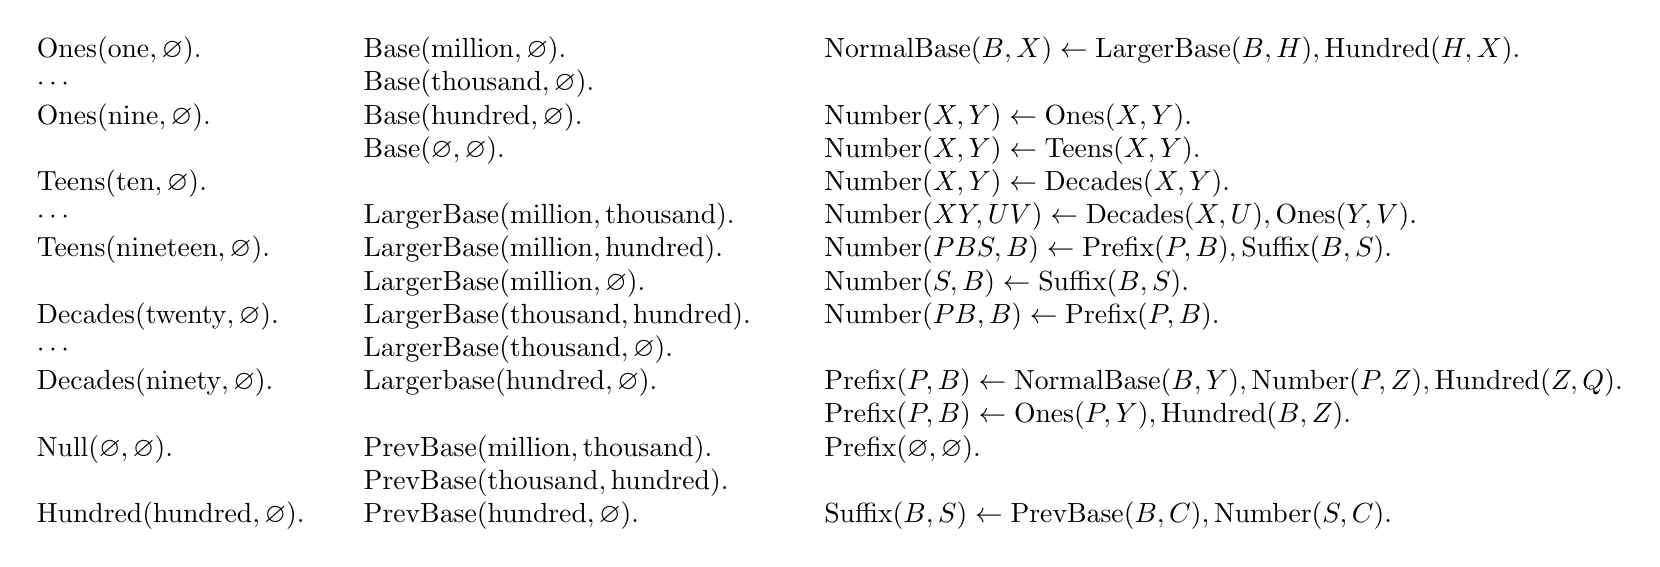
\begin{tikzpicture}[scale=1,every text node part/.style={align=left}]
  \tikzstyle{vertex}=[circle,draw,minimum size=19pt,
    inner sep=1pt, outer sep=1pt]
  
  \node [anchor=north west] (desc) at (0,0) {
    $\text{Ones}(\text{one}, \varnothing).$\\
    $\cdots$\\
    $\text{Ones}(\text{nine}, \varnothing).$\\
    \\
    $\text{Teens}(\text{ten}, \varnothing).$\\
    $\cdots$\\
    $\text{Teens}(\text{nineteen}, \varnothing).$\\
    \\
    $\text{Decades}(\text{twenty}, \varnothing).$\\
    $\cdots$\\
    $\text{Decades}(\text{ninety}, \varnothing).$\\
    \\
    $\text{Null}(\varnothing,\varnothing).$\\
    \\
    $\text{Hundred}(\text{hundred}, \varnothing).$
  };
  \node [anchor=north west] (desc) at (4.15,0) {
    $\text{Base}(\text{million}, \varnothing).$\\
    $\text{Base}(\text{thousand}, \varnothing).$\\
    $\text{Base}(\text{hundred}, \varnothing).$\\
    $\text{Base}(\varnothing, \varnothing).$\\
    \\
    $\text{LargerBase}(\text{million}, \text{thousand}).$\\
    $\text{LargerBase}(\text{million},\text{hundred}).$\\
    $\text{LargerBase}(\text{million}, \varnothing).$\\
    $\text{LargerBase}(\text{thousand},\text{hundred}).$\\
    $\text{LargerBase}(\text{thousand},\varnothing).$\\
    $\text{Largerbase}(\text{hundred}, \varnothing).$\\
    \\
    $\text{PrevBase}(\text{million}, \text{thousand}).$\\
    $\text{PrevBase}(\text{thousand}, \text{hundred}).$\\
    $\text{PrevBase}(\text{hundred}, \varnothing).$
  };
  \node [anchor=north west] (desc) at (10,0) {
    $\text{NormalBase}(B,X) \leftarrow \text{LargerBase}(B,H), \text{Hundred}(H,X).$\\
    \\
    $\text{Number}(X,Y) \leftarrow \text{Ones}(X,Y).$\\
    $\text{Number}(X,Y) \leftarrow \text{Teens}(X,Y).$\\
    $\text{Number}(X,Y) \leftarrow \text{Decades}(X,Y).$\\
    $\text{Number}(X Y,U V) \leftarrow \text{Decades}(X,U), \text{Ones}(Y,V).$\\
    $\text{Number}(P B S,B) \leftarrow \text{Prefix}(P,B), \text{Suffix}(B,S).$\\
    $\text{Number}(S,B) \leftarrow \text{Suffix}(B,S).$\\
    $\text{Number}(P B,B) \leftarrow \text{Prefix}(P,B).$\\
    \\
    $\text{Prefix}(P,B) \leftarrow \text{NormalBase}(B,Y), \text{Number}(P,Z), \text{Hundred}(Z,Q).$\\
    $\text{Prefix}(P,B) \leftarrow \text{Ones}(P,Y), \text{Hundred}(B,Z).$\\
    $\text{Prefix}(\varnothing, \varnothing).$\\
    \\
    $\text{Suffix}(B,S) \leftarrow \text{PrevBase}(B,C), \text{Number}(S,C).$
  };
\end{tikzpicture}
\end{document}
